%!TEX root=report.tex
\subsection{Least angular regression (LAR)}
\label{section:result-lar}

The full solution path is in this case very hard to interpret, so instead the relative coefficients are shown. That is the coefficients at an iteration divided by the final value (the plain OLS case).

\begin{figure}[H]
	\centering
	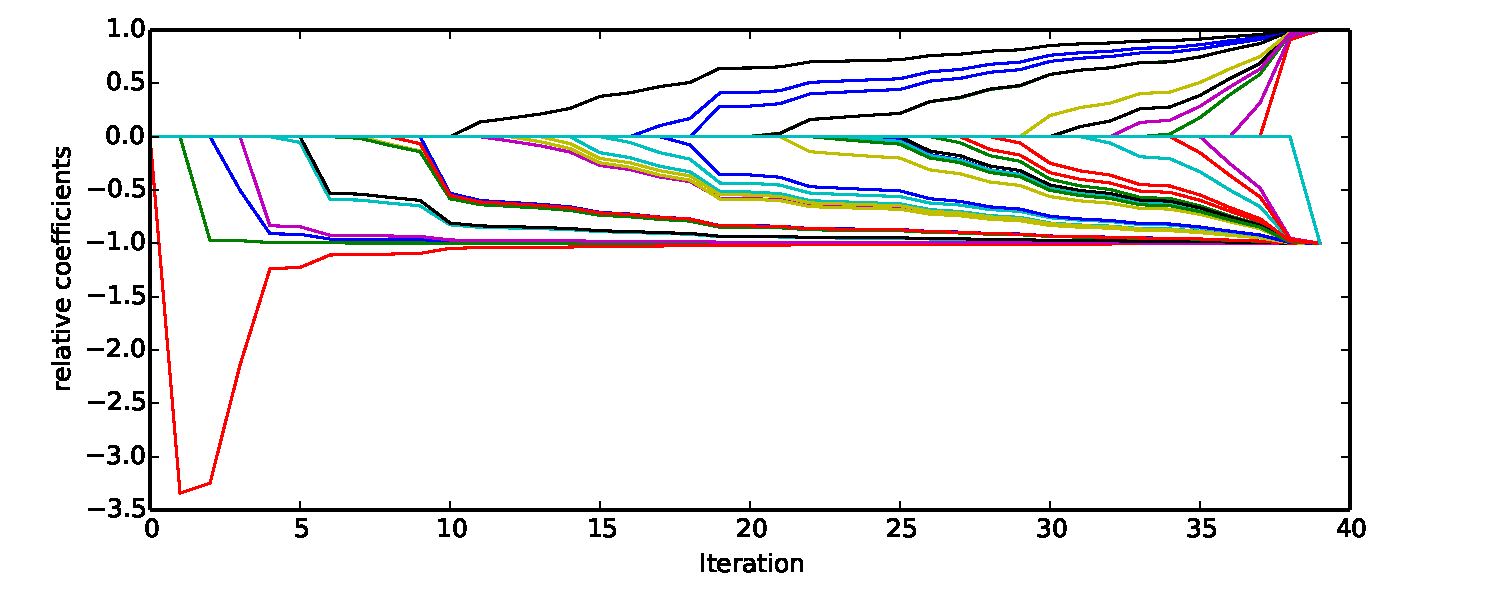
\includegraphics[width=\textwidth]{figures/lar-coefficients}
	\caption{The full solution path shown with relative coefficients. Position is 63.5 N 49.5 W, west coast of Greenland.}
	\label{fig:lar-coefficients}
\end{figure}

From Figure \ref{fig:lar-coefficients} it appears that the first 7 coefficients are the more relevant. 
\begin{table}[H]
\centering
\begin{tabular}{r|l}
name                 & coeffecients \\ \hline
intercept ($1$) & $-1.69 \cdot 10^{-1}[m]$ \\
velocity ($t$) & $-2.23 \cdot 10^{-4} [\sfrac{m}{day}]$ \\
acceleration ($0.5 \cdot t^2$) & $-9.16 \cdot 10^{-8} [\sfrac{m}{day^2}] $ \\
$\cos(2 \pi /365.2 * t)$ & $-8.06 \cdot 10^{-3}$ \\
$\sin(2 \pi /365.2 * t)$ & $-7.67 \cdot 10^{-2}$ \\
$\sin(2 \pi /182.6 * t)$ & $-7.59 \cdot 10^{-3}$ \\
$\sin(2 \pi /121.7 * t)$ & $-8.67 \cdot 10^{-5}$
\end{tabular}
\caption{LAR coefficients in the seventh iteration}
\end{table}

Using these seven coefficients the following line $\hat{y}$ can be calculated:
\begin{figure}[H]
\center
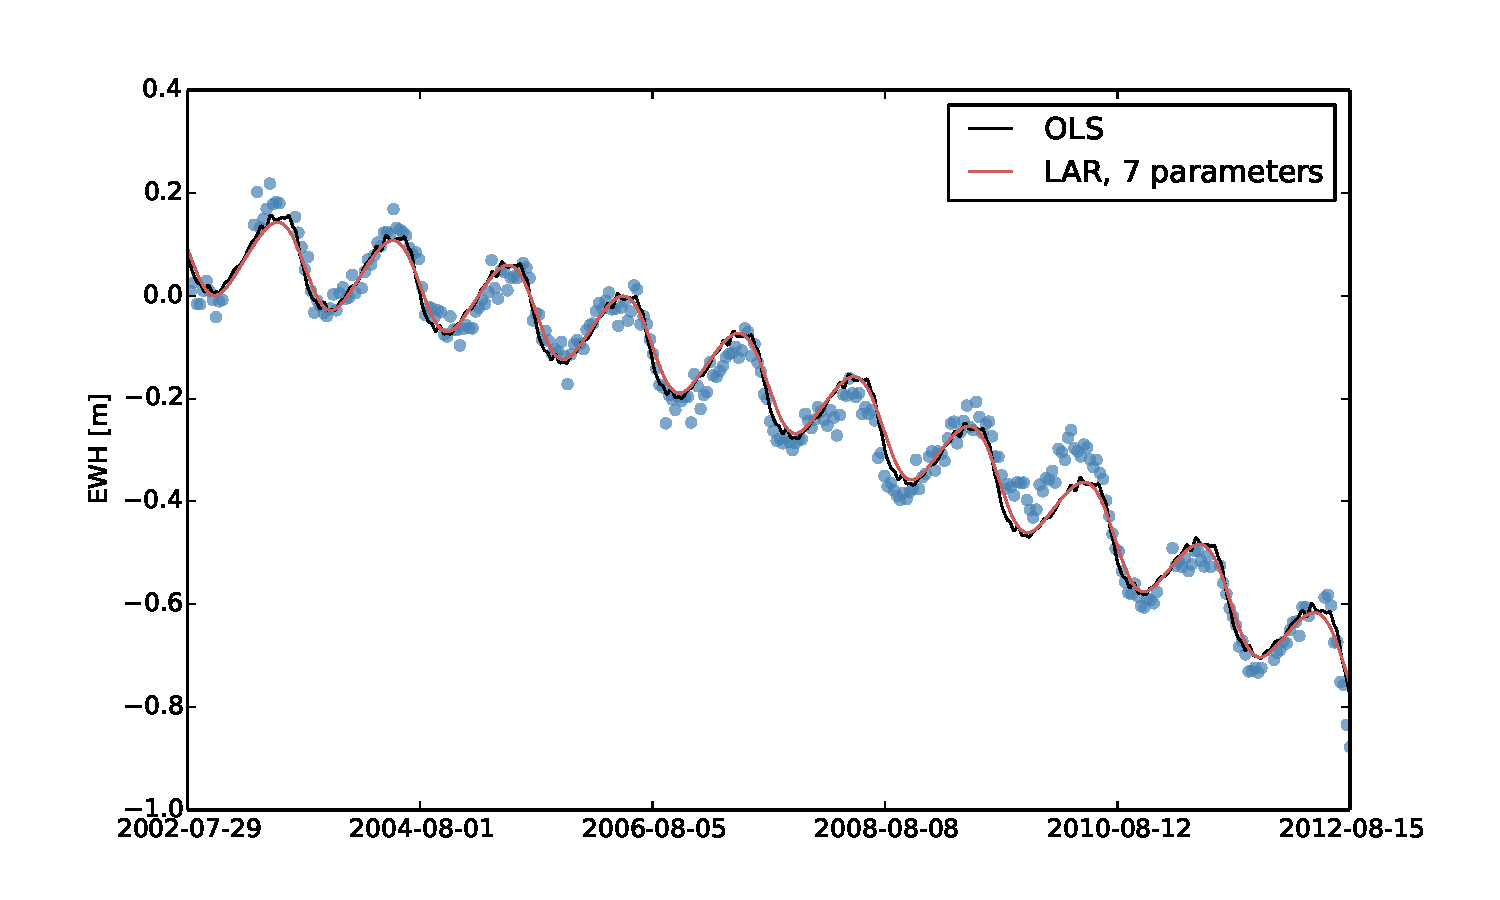
\includegraphics[width=\textwidth]{figures/lar-compare}
\caption{OlLS and LAR (seven parameters) compared. Position is 63.5 N 49.5 W, west coast of Greenland.}
\end{figure}

\subsubsection{How many frequencies are actually needed}

This was done for one position on the globe only. If one were to apply this to other positions one might get different lasso-paths and perhaps also a slight variation in the number of coefficients needed. For example for modeling the ocean one would not need as many coefficients, while at places with heavy rain season such as South America, more coefficients might be needed.
